%%%%%%template by Daniel Parker
%%%%%%http://dug.math.brown.edu/
\documentclass[10pt,twoside]{article}
%%%%%%%%%packages%%%%%%%%%
\usepackage{amsmath}
\usepackage{amssymb}
\usepackage{amsfonts}
\usepackage{amsthm}
\usepackage{mathrsfs}
\usepackage{mathtools}
\usepackage{colonequals} 	
\usepackage{graphicx}
\usepackage{fancyhdr}
\usepackage{multirow}
\usepackage{siunitx}
\usepackage{tikz}
\usepackage[headings]{fullpage}

%%%%%%%%%header%%%%%%%%%
\pagestyle{fancy}
\fancyhead{} % clear all header fields
\renewcommand{\headrulewidth}{0.2pt}
\fancyhead[RO,LE]{\bfseries \hspace{1in}\rightOne\phantom{\hspace{1in}}\\ \hspace{1in}\rightTwo\hspace{1in}}
\fancyhead[RE,LO]{\bfseries \hspace{1in}\leftOne\phantom{\hspace{1in}}\\ \hspace{1in}\leftTwo\hspace{1in}}
\fancyhead[C]{\bfseries \centerOne\\\centerTwo}
\fancyfoot{}
\setlength{\voffset}{-1in+1.5em}
\fancyheadoffset{1in}
\addtolength{\textheight}{1in}

%%%%%%%%%theorem environment and numbering%%%%%%%%%
%%%%%%%%%uses amsthm package
\newtheorem{thm}{Theorem}
\newtheorem{prop}[thm]{Proposition}
\newtheorem{lm}[thm]{Lemma}
\newtheorem{defn}[thm]{Definition}
\newtheorem{rem}[thm]{Remark}
\newtheorem{cl}{Claim}[thm]
\newtheorem{cor}[thm]{Corollary}

\theoremstyle{definition}
\newtheorem{eg}[thm]{Example}

%%%%%%%%%exercise numbering%%%%%%%%%
\newtheoremstyle{exercise}{}{}{\itshape}{}{\bfseries}{:}{.5em}{\thmname{#1} \thmnumber{#2}\thmnote{(#3)}}
\theoremstyle{exercise}
\newtheorem{ex}{Exercise}
\newcommand{\nextex}[1]{\begin{ex}\end{ex}}
\newcommand{\nextexP}[1]{\begin{ex}#1\end{ex}}
\newcommand{\setex}[1]{\setcounter{ex}{#1-1}\begin{ex}\end{ex}}
\newcommand{\setexP}[2]{\setcounter{ex}{#1-1}\begin{ex}#2\end{ex}}

%%%%%%%%%notation shortcuts%%%%%%%%%
\newcommand{\R}{\mathbb{R}}
\newcommand{\Q}{\mathbb{Q}}
\newcommand{\Z}{\mathbb{Z}}
\newcommand{\N}{\mathbb{N}}
\newcommand{\F}{\mathbb{F}}
\newcommand{\C}{\mathbb{C}}


\newcommand{\n}[1]{\left| #1 \right|}%%adjustable-height norm shortcut
\newcommand{\set}[2]{\left\{#1\left|\; #2 \right. \right\}}%%set notation shortcut with a line
\newcommand{\setc}[2]{\left\{#1\; :\; #2 \right\}}%%set notation shortcut with a colon
\newcommand{\st}[1]{\left\{#1\right\}}%%set notation shortcut with no condition
\newcommand{\ce}{\colonequals}%%shortcut to write \colonequals

\newcommand{\bvi}{\hat{\mathbf{i}}} %basis vector i
\newcommand{\bvj}{\hat{\mathbf{j}}} %basis vector j
\newcommand{\bvk}{\hat{\mathbf{k}}} %basis vector k
\newcommand{\bvr}{\hat{\mathbf{r}}} %basis vector r
\newcommand{\bvt}{\hat{\mathbf{\theta}}}%basis vector theta
\newcommand{\bvx}{\hat{\mathbf{x}}} %basis vector x
\newcommand{\bvy}{\hat{\mathbf{y}}}%basis vector y
\renewcommand{\v}[1]{\mathbf #1}%%shortcut to make a vector N.B. this overwrites the default command for \v which makes a caret over the letter

\newcommand{\aut}{\operatorname{Aut}}
\newcommand{\mor}{\operatorname{Mor}}
\newcommand{\chr}{\operatorname{char}}
\newcommand{\spn}{\operatorname{span}}
\newcommand{\tr}{\operatorname{Tr}}
\newcommand{\im}{\operatorname{Im}}


%%%MODIFY THESE LINES TO CHANGE THE HEADER
\newcommand{\leftOne}{Brown University}
\newcommand{\leftTwo}{Prof. Dell'Antonio}
\newcommand{\centerOne}{Overview and Technical Description of \texttt{jedisim}}
\newcommand{\centerTwo}{26 July  2013}
\newcommand{\rightOne}{\thepage}
\newcommand{\rightTwo}{Dan Parker}

\begin{document}
\section{Purpose}

Gravitational Lensing provides an accurate way to determine the mass distribution of objects based solely on the mass present, and is impartial to the details of how the mass interacts. Lensing is therefore ideal to study the mass distributions of galaxy clusters, which are often surrounded by dark matter halos. Moreover, since lensing is an independent measurement, it can be used to calibrate other measurement techniques such as x-ray emission or velocity dispersion measurements.  

  However, gravitational lensing measurements of mass distributions are subject to the same pitfalls as all observational science. Namely, it is tricky to determine the magnitude and sources of errors in measurement. If there were a ``perfect'' galaxy cluster whose mass distribution was known exactly, then it would be easy to quantify errors in the lensing measurement by comparing to that standard. Of course, no such ``perfect'' clusters exist. Therefore, the best alternative is to \textit{simulate} a ``perfect'' cluster and use it to determine and minimize errors.



\section{Overview}

Any simulation is only as accurate as the model and parameters used to create it. Indeed, systemic inaccuracies in error measurements are inevitably introduced by whatever differences exist between the simulation and actual galaxy clusters. The best way to counteract this and reduce inaccuracies is to make the model and its parameters as physically accurate as possible. This, in turn, is limited by the computational power available and the precision of the parameters used to calibrate the model. Judicious selection of what approximations and simplifications are used is required to make the model. Equally important is the amount of control a model affords: all parameters can be adjusted and phenomena can be turned on or off as desired. This allows the importance and effect of parameters to be studied individually. This report details and explains the \texttt{jedisim} model and its parameters.

The \texttt{jedisim} simulation models the effect of a foreground galaxy cluster on the shapes of background galaxies. There are three main components of the simulation:
\begin{enumerate}
  \item Creating a field of background galaxies.
  \item Distorting the light from the background galaxies in accordance with a specified mass distribution.
  \item Blurring and distorting the light to mimic the effects of Earth's atmosphere and the optical properties of a telescope. 
\end{enumerate}
The three steps are performed as independently as possible so that the model can be improved in a modular fashion. An effort is made to simulate galaxies individually and not combine them into a single image as late as possible so that redshift-dependent effects can be included. Furthermore, the simulation is done across a very wide area of the sky --- a 1200 by 1200 arcsecond square, or $>2$ Mpc at $z = 0.3$ --- which is large enough that measurement of lensing signal is not limited by the image size, but small enough that it can be treated as flat, i.e. the pixels are square. In the final step of the simulation, images are created as they would be observed by the upcoming LSST telescope (6000 by 6000 pixels at $0.2$ arcseconds per pixel). To ensure that there are no pixelation effects, the first two steps are carried out at HST UDF resolution with a $\sim$30 arcsecond border to surpress edge effects, which gives an image size of 40960 by 40960 pixels at $0.03$ arcseconds per pixel. 

The parameters and models for each step in the simulation are discussed in the next three sections, along with relevent implementation details. 

\section{Simulating A Galaxy Field}
\label{sec:background}
The background galaxy field is simulated one galaxy at a time. Individual galaxies are taken from an HST UDF image and converted to 600 by 600 pixel ``postage stamps'' images where the galaxy is isolated on a blank background --- see Figure \ref{fig:postage_stamp}. We regard these as truth images. All the postage stamps are at the drizzled UDF resolution of 0.03 arcseonds per pixel. The Hubble PSF was not removed since noise from deconvolution can be magnified greatly by strong lensing effects, creating unrealistic galaxy shapes. The slight bias in shape added by the Hubble PSF is negligible because the size of most of the galaxies is much larger than the size of the PSF, and galaxies of all orientations are used. The sample of 128 postage stamps is large enough that there is a fairly diverse set of galaxy shapes and orientations.

\begin{figure}
  \begin{center}
    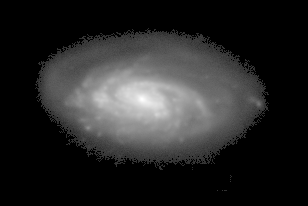
\includegraphics[scale=10]{../images/example_galaxy.png}
  \end{center}
  \caption{An example ``postage stamp'' galaxy at a log scale.}
  \label{fig:postage_stamp}
\end{figure}


We simulated galaxies ranging from 22\textsuperscript{nd} to 28\textsuperscript{th} magnitude. When the sky is observed, a significant number of galaxies at these magnitudes will be both extended and relatively faint. Benitez et al. (FAINT GALAXIES IN DEEP ACS OBSERVATIONS) point out that the measured number density of galaxies will be biased low because some galaxies are rendered indistinguishable from the background by the noise level. Using deep HST images, they estimate the an average ?? by ?? arcsecond patch of the sky will have ???? detectable galaxies and ???? additional undetectable ones. Extrapolating to 1200 by 1200 pixels, we will simulate a total of $138,000$ galaxies of which $\sim40,000$ will be detectable. However, with strong enough lensing, some of the undetectable galaxies will be magnified enough that they can be isolated from the background. This bias in the number density and magnitude of galaxies near cluster has been observed in [???, I hope it's actually been observed!] and will be accurately included in this simulation. The galaxies which remain undetectable even with lensing, add realistic cosmic background light to the images.

Each galaxy is specified by six parameters detailed below.

\begin{description}
  \item[Magnitude] The magnitude M of each galaxy is selected in the range $22 \le M \le 28$ with the distribution given by the power law
    \begin{equation}
      P(M+dM) \propto 10^{BM}
      \label{eq:mag_power_law}
    \end{equation}
    where $M$ is the magnitude and $B = 0.33\ln 10$ is an emperical constant.[Benitez et al.] The magnitude zero-point is taken to be 30 throughout the simulations by convention.

  \item[Radius] 
For each galaxy, an r50 radius is selected from the database of r50 galaxy radii in [Kubo et al, from HDF catalogs]. Specifically, the database is binned by the integer part of the magnitude  and a list of radii is made for each magnitude. Since each postage stamp is already assigned a magnitude, it has a corresponding bin, and an r50 radius is chosen randomly from that bin.

  \item[Image] A postage stamp image is chosen at random from the postage stamps whose r50 value is larger than the r50 assigned to the galaxy. This is done so that images are always sized down, so no information is artificially created by scaling.

  \item[Redshift] The database of galaxy redshift from [cite ZCOSMOS database] is used and, as with radius, binned by integer magnitude. For each galaxy, a redshift is selected from the corresponding magnitude bin. Alternatively, a single redshift (i.e. $z=1.5$) can be chosen for all galaxies.

  \item[Position] The center of the postage stamp is selected as a pair of uniformly distributed floating points (for $x$ and $y$ position) from the range $[301, 40660]$. This range is taken to ensure that all 600 by 600 postage stamp images lie completely within the range $[0,40960]$. In a later step, (See Section \ref{sec:atmospherics}) a border of size $480$ is trimmed from each side of the image, ensuring a uniform distribution of galaxy positions with typical edge effects, i.e. some galaxies are partially sliced off by the edge of the image. In principle, the background galaxies are clustered, but this has not been implemented.

  \item[Angle] 
  Each galaxy is randomly oriented by choosing an an angle uniformly from the range $[0,2\pi)$. 
  
  An angle is chosen uniformly in the range $[0,360)$ through which the postage stamp will be rotated. This is to ensure the orientation of the galaxies is random. The orientation of galaxies has at least three degrees of freedom, but since we are dealing with 2D projections of galaxies, we can only make the orientation random in one degree of freedom, with some additional variability coming from the diverse orientations of the postage stamps. 
\end{description}

Once these parameters are chosen for each galaxy, an image is made which satisfies those parameters. Specifically, the postage stamp is scaled down to the correct r50 radius, rotated through the assigned angle (using a bilinear interpolation), and its flux is adjusted to the correct magnitude. The galaxy is then cut out, so that the image consists of the smallest rectangle that contains all non-zero pixels of the galaxy. Each transformed postage stamp galaxy is saved as a FITS image together with the 6 parameters which characterize it.

We now have all the information for the background image: a catalog of galaxies whose sizes, magnitudes, orientations, positions and (optionally) redshifts are distributed in accordance with cosmic observations.

\section{Simulating Gravitational Lensing}
\begin{figure}[h]
		\begin{center}
          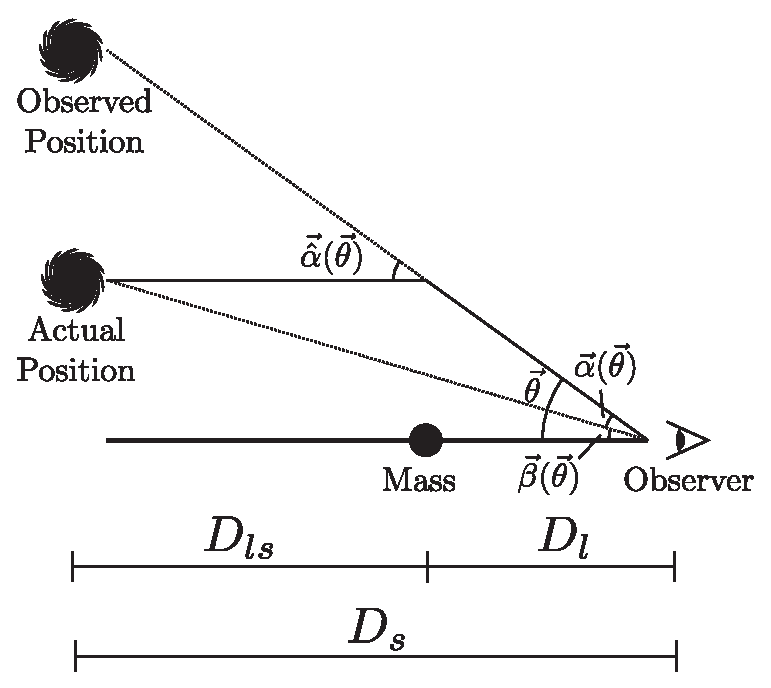
\includegraphics[scale=0.5]{../images/lensing_formalism.eps}
		\end{center}
		\caption{Diagram of gravitational lensing.}
		\label{fig:lensing_diagram}
\end{figure}


\subsection{Model}
The next step in the simulation is to emulate the effects of gravitational lensing caused by a galaxy cluster. In the weak field limit, for a point mass, this is governed by the Lens Equation
\begin{equation}
  \vec{\beta}(\vec{\theta}) = \vec{\theta} - \vec{\alpha}(\vec{\theta}) = \vec{\theta} - \frac{D_{ls}}{D_s}\vec{\hat{\alpha}}(\vec{\theta})
  \label{eq:lensing}
\end{equation}
where $\vec{\beta}$ is the angle between the light source and the point mass, $\vec{\theta}$ is the angle between the point mass and the apparent position of the light source, $\vec{\alpha}(\vec{\theta})$ is the deflection angle of the light at $\vec{\theta}$, $\vec{\hat{\alpha}}(\vec{\theta})$ is the corresponding unit vector, and $D_{ls}$ and $D_s$ are the angular diameter distance from the lens to the source and the observer to the source respectively. (See Figure \ref{fig:lensing_diagram}.) The deflection $\vec{\hat{\alpha}}$ is a vector quantity and, assuming the weak field limit, the deflections from a distribution of mass add linearly.


For computational simplicity, the gravitational lens is specified as a radially symmetric mass distribution with the center at an arbitrary location and arbitrary redshift. The deflection term in the Lens Equation then becomes
\begin{equation}
  \vec{\hat{\alpha}}(\vec{\theta}) = \alpha(r) \vec{\hat{r}}
  \label{eq:rad_symm_lens_eq}
\end{equation}
where $\alpha(r)$ is the radial deflection which depends on the mass distribution, $r$ is the distance from the center of the mass distribution to $\vec{\theta}$, and $\vec{\hat{r}}$ is the unit vector from the center of the mass distribution to $\vec{\theta}$. Both $r$ and $\alpha(r)$ have units of pixels. The two lensing mass distributions implemented in \texttt{jedisim} are described below.
\begin{description}
  \item[Singular Isothermal Sphere (SIS) Profile] The SIS profile is one of the simplest models of the mass distribution of a galaxy cluster.[cite] Its density is given by
    \begin{equation}
      \rho(r; \sigma_v) = \frac{\sigma_v^2}{2\pi Gr^2}
      \label{eq:SIS_density}
    \end{equation}
    where $\sigma_v$ is the velocity dispersion and $G$ is the universal gravitational constant. Since the total mass inside radius $r$ diverges as $r \to \infty$, the SIS profile is non-physical. However, as long as the profile is finitely bounded, it constitutes a possible physical distribution and can be used as a lens. The deflection in pixels due to an SIS profile is given by 
    \begin{equation}
      \frac{\alpha(r; \sigma_v)}{r} = \frac{4\pi}{r}\left( \frac{\sigma_V}{c} \right)^2S
      \label{eq:SIS_deflection}
    \end{equation}
    where $r$ is the radius in pixels, $\sigma_v$ is the dispersion parameter in km/s, $c$ is the speed of light in km/s, and $S$ is the conversion factor between pixels and radians given by
    \begin{equation}
      S = \frac{\pi}{180}\frac{3600}{\text{resolution}}
      \label{eq:px_per_rad}
    \end{equation}
    where ``$\text{resolution}$'' is the resolution of the image in arcseconds per pixel.

  \item[Navarro-Frenk-White (NFW) Profile] The NFW profile was discovered to emperically fit $N$-body simulations of galaxy clusters.[cite NFW's 1997 paper ``A Universal Density Profile from Hierarchical Clustering''] The NFW profile can be expressed in several different ways depending on what parameters are used. In the most common form, the density of the NFW profile is given by
    \begin{equation}
      \rho(r; \delta_c, R_s) = \frac{\rho_\text{crit}\delta_c}{\dfrac{r}{R_s}\left( 1+\dfrac{r}{R_s} \right)^2}
      \label{eq:NFW_density}
    \end{equation}
    where $\rho_\text{crit}$ is the critical density for closure [what does this mean?] given by
    \begin{equation}
      \rho_\text{crit} = \frac{3H^2}{8\pi G},
      \label{eq:rho_crit}
    \end{equation}
    $\delta_c$ is a dimensionless density parameter, and $R_s$ is a scale radius. Another way to describe the NFW profile is by its virial radius and mass. Let $r_{200}$ be the virial radius of the cluster. Then we define a dimensionless concentration parameter of the cluster by
    \begin{equation}
      c = \frac{r_{200}}{R_s}.
      \label{eq:concentration_parameter}
    \end{equation}
By the definition of virial radius, the density parameter can be rewritten in terms of the concentration parameter:
    \begin{equation}
      \delta_c = \frac{200}{c} \frac{c^3}{\ln(1+c)-\frac{c}{1+c}}.     
      \label{eq:delta_c}
    \end{equation}
Furthermore, the virial mass can be written as
\begin{equation}
  M_{200} = 4\pi\rho_\text{crit}\delta_cR_s^3\left[ \ln(1+c) - \frac{c}{1+c} \right].
  \label{eq:virial_mass}
\end{equation}
    These two parameters are much more natural to use when describing the cluster. $M_{200}$ is often calculated when finding cluster masses, and $c$ is widely used as a parameter in cluster simulations. It is then possible (but ugly) to express the density as $\rho(r; M_{200}, c)$.

    The deflection in pixels by the NFW profile is given by
    \begin{equation}
      \frac{\alpha(r; M_{200}, c)}{r} \ =  \frac{4GM_{200}\delta'_c}{9\times 10^5 D_L\, r} \times \left[\log \frac{x}{2} +  
      \begin{cases}
        \frac{2}{\sqrt{1-x^2}}\operatorname{arctanh}\left( \sqrt{\frac{1-x}{1+x}} \right) & \text{ if $x \in (0, 1)$}\\
        1 & \text{ if $x=1$}\\
        \frac{2}{\sqrt{x^2-1}}\arctan\left( \sqrt{\frac{x-1}{1+x}} \right) & \text{ if $x > 1$.}\\
      \end{cases}
      \right]
      \label{eq:NFW_deflection}
    \end{equation}
    where $r$ is the radius in pixels, $M_{200}$ is the virial radius, $c$ is \textit{not} the speed of light, but rather a unitless concentration parameter for the NFW profile, $G$ is the universal gravitational constant with value $G = 4.302$ in these units, $D_L$ is the angular diameter distance of the cluster for a given cosmology, $S$ is the conversion factor given in Equation $\eqref{eq:px_per_rad}$, $\delta'_c$ is a slight modification of the density parameter, 
    \begin{equation}
      \delta'_c = \frac{1}{\log(1+c)-\frac{c}{1+c}},
        \label{eq:mod_delta_c}
    \end{equation}
    and $x$ is a unitless distance variable given by
    \begin{equation}
      x = \frac{Sc D_L}{10.0}\left(\frac{G}{H_0^2}\right)^{-1/3}r
      \label{eq:unitless_x}
    \end{equation}
    where $H_0$ is the Hubble constant at the present time, and $c$ is the concentration parameter.
\end{description}

An arbitrary number of lenses may be present simultaneously, whose type (SIS or NFW), center point, redshift, and profile parameters are all specified by a configuration file. In the current implementation, the redshift of all lenses must be the same. The deflection then becomes the superposition of the deflections from each of the lenses: if there are $N$ lenses with deflection functions $\alpha_i$ for $i = 1,\dots, N$, then the deflection term becomes
\begin{equation}
  \vec{\hat{\alpha}}(\vec{\theta}) = \sum_{i=1}^N \alpha_i(r_i) \vec{\hat{r}}_i
  \label{eq:superposition_lens_eq}
\end{equation}
where $r_i$ is the distance between and unit vector from the center of the $i$\textsuperscript{th} mass distribution to $\vec{\theta}$, respectively.


The lensed image is calculated by applying Equation $\eqref{eq:rad_symm_lens_eq}$ to the background image produced in Section \ref{sec:background}. This is done as follows. For now, assume that all background galaxies lie at a single redshift. Then we can consider the universe as three parallel planes: the source plane where the background galaxies lie, the lens plane where the mass distribution lies, and the observation plane which is near earth but above the atmosphere.

Any light going from the source plane to the observation plane will pass through the lens plane and be deflected, forming a distorted image of the source plane on the observation plane. The na\"ive way to determine what this distorted image will be is to trace the path of individual photons from the source image to the observation image. Unfortunately, this is non-deterministic because of the phenomena of multiple images, and is thus extremely inefficient. However, it is possible to go backwards. Concretely, let $I$ and $J$ be the scalar-valued intensity function on the source and observation planes respectively and let $\vec{\hat{\alpha}}$ be the vector-valued deflection function on the lens plane. Then with $\vec{\theta} = (x, y)$,
\begin{equation}
  J(x,y) = I\left( \vec{\beta}(x,y)\right) = I\left( (x,y)- \frac{D_{ls}}{D_s} \vec{\hat{\alpha}}(x,y) \right).
  \label{eq:lens_intensity_eq}
\end{equation}
This equation contains the assumption from above that all background objects have a single redshift. In the (more realistic) case where there are background galaxies at multiple redshifts, there is a separate source plane for each redshift, and a corresponding observation plane can be calculated for each one. The total observation intensity is just the sum over all these planes.


\subsection{Implementation Details}
In this simulation, the source and observation planes are not really planes, but rather finite lattices with side length 40690. Let $\tilde{I}$ and $\tilde{J}$ as the intensity functions on those lattices. Also let $\texttt{round}$ be a function which takes a 2-dimensional vector and returns the closest lattice point. Then we can production a discrete version of Equation $\eqref{eq:lens_intensity_eq}$:

\begin{equation}
  \tilde{J}(x,y) = \tilde{I}\left( \texttt{round}\left( \vec{\beta}(x,y) \right)\right) = \tilde{I}\left(\texttt{round} \left( (x,y)- \frac{D_{ls}}{D_s} \vec{\hat{\alpha}}(x,y)  \right)\right).
  \label{eq:discrete_lens_intensity_eq}
\end{equation}
With large densities, $\vec{\hat{\alpha}}$ can change significantly over a single pixel. It is therefore necessary to use \textit{subpixel} precision: each pixel is chopped up into a grid and its value is set to the average of the values computed for each subpixel. We then define $\tilde{J}_n(x,y)$, the intensity function on the observation lattice with subpixel size n, as
\begin{equation}
  \tilde{J}_n(x,y) = \frac{1}{n^2}\sum_{i=0}^{n-1}\sum_{j=0}^{n-1} \tilde{I}\left( \texttt{round}\left( \vec{\beta}(x+i\Delta,y+j\Delta) \right)\right)
  \label{eq:discrete_subpixel_lens_intensity_eq}
\end{equation}
where $\Delta = 1/n$. As currently implemented, \texttt{jedisim} uses $n=4$.

In theory, this does it. For each galaxy, we can form a source lattice and calculate $\tilde{J}_4(x,y)$ for each pixel $(x,y)$. However, this is a total of $2.3 \times 10^{14}$ pixels, which makes for an impractically long computation, particularly with subpixel accuracy. Luckily, most of these computations are unnecessary. Each galaxy is tiny --- the image for each galaxy is usually about 30 by 30. Even with the large magnifications sometimes seen with strong lensing, the image of each galaxy in the observation plane will only have a few thousand non-zero datapoints. If we knew \textit{a priori} where those pixels were, it would only be necessary to do a few thousand computations per galaxy instead of $40960^2$ computations. The algorithm for finding those pixels, without calculating the whole image, is detailed below. It is quite efficient, but somewhat involved.

First, a useful definition is needed. Consider an image that is mostly blank (most pixels have zero intensity). Define the \textit{information box} of the image to be the minimal rectangle that contains all non-blank pixels.  The image age is completely specified by the position and contents of its information box.


The information box of a background galaxies $G$ is a region $R_G$ in the source plane. Let $O(R_G)$ be the region of the observation plane where light from $R_G$ ends up after passing through the lens. So to calculate $\tilde{J}_4$ over the entire observation plane, it is sufficient to calculate it over $O(R_G)$. Since $O(R_G)$ is much smaller than the whole image --- usually by five or six orders of magnitude --- this is a much faster way to find $\tilde{J}_4$.

It is computationally impractical to compute $O(R_G)$ by ray tracing light from $R_G$. Instead, we search for a slightly larger region $O^+(R_G)$ that can be found quickly. $O^+(R_G)$ is found by an algorithm given below. First several necessary definitions must be made.


Let $S_N$ be a \textit{square-covering} of size $N$ of the observation plane, a set of squares with sidelength $N$ that make a ``checkerboard'' over the observation plane. See Figure \ref{fig:checkerboard}. Of course, this can be only defined when $N$ divides the side length of the observation plane, 40960. Let $X$ and $Y$ be coordinates on the squares. Because the covering is finite, they range from $0$ to $(40960/N)-1$ inclusive.

\begin{figure}[h]
		\begin{center}
				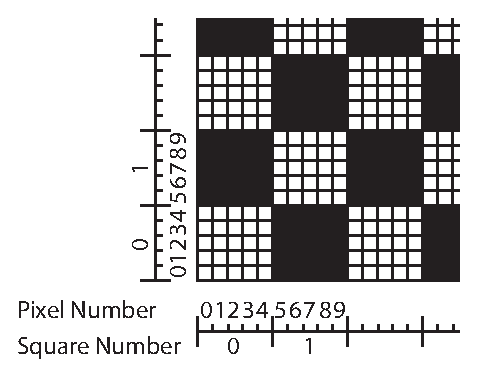
\includegraphics[scale=0.7]{../images/checkerboard.eps}
		\end{center}
		\caption{Diagram of a square covering with $N=5$. }
		\label{fig:checkerboard}
\end{figure}

For a square-covering $S_N$, define $B_N(X, Y)$ to be a 4-tuple-valued function on $S_N$ where each 4-tuple gives the minimum and maximum values of both components of $\vec{\hat{\alpha}}(x,y)$ over the square $(X,Y)$. Concretely, $B_N(X,Y)$ is given by
\begin{equation}
  B_N(X,Y) = \begin{pmatrix}
    \displaystyle\min_{(x,y) \in S}\left[\vec{\hat{\alpha}}(x,y)\right]_x \\
    \displaystyle\max_{(x,y) \in S}\left[\vec{\hat{\alpha}}(x,y)\right]_x \\
    \displaystyle\min_{(x,y) \in S}\left[\vec{\hat{\alpha}}(x,y)\right]_y \\
    \displaystyle\max_{(x,y) \in S}\left[\vec{\hat{\alpha}}(x,y)\right]_y
  \end{pmatrix}
  \label{eq:alpha_box}
\end{equation}
where $S$ is the set of all pixels inside the square $(X,Y)$, i.e.
\begin{equation}
  S = \setc{(x,y)}{NX \le x < N(X+1),\quad NY\le x N(Y+1)}
  \label{eq:pix_in_sqaure}
\end{equation}
For a specific square $(X,Y)$ in the observation plane and a specific galaxy, define the \textit{pullback information box}, $\text{PIB}(X,Y)$, as the maximal rectangle in the source plane where information can be drawn from when computing $\tilde{J}_4$ over the square. When described by its edges, i.e. its $x$ and $y$ minima and maxima respectively, the pullback information box is given by
\begin{equation}
  \text{PIB}(X_N,Y_N; D_{ls}, D_{s}) = \begin{pmatrix}
    N(X_N+1)-1-\dfrac{D_{ls}}{D_s}B(X,Y)_1\\
    NX_N-\dfrac{D_{ls}}{D_s}B(X,Y)_2\\
    N(Y_N+1)-1-\dfrac{D_{ls}}{D_s}B(X,Y)_3\\
    NY_N-\dfrac{D_{ls}}{D_s}B(X,Y)_4\\
  \end{pmatrix}
  \label{eq:pullback_square_infobox}
\end{equation}
where $B(X_N,Y_N)_i$ is the $i$\textsuperscript{th} component of $B(X_N,Y_N)$, and $D_{ls}$ and $D_{s}$ are distances that depend on the galaxy. Then, for a specific galaxy, we can check if the box defined by $PIB(X_N,Y_N; D_{ls}, D_s)$ intersects $R_G$ in the source plane. If they do not intersect, then $\tilde{J}_4$ vanishes over $(X,Y)$. If they do intersect, then $\tilde{J}_4$ may not vanish over $(X,Y)$.

\begin{figure}[h]
		\begin{center}
				\includegraphics[scale=1]{../images/algorithm.eps}
		\end{center}
		\caption{Step 5 of the algorithm for two squares. Left side: case of no intersection between pullback information box and Galaxy information box. Right side: case of intersection.}
		\label{fig:algorithm}
\end{figure}

With these definitions, we can give the algorithm to find $O^+(R_G)$.
\begin{enumerate}
  \item Make the square-covering $S_N$ for $N = 8, 64, 512, 4096$. Notice that these are ``nested'': each square contains 64 sub-squares inside it, except for the square in $S_8$, which contain $64$ pixels each.
  \item Compute $B_N(X_N,Y_N)$ for each $N$. 
  \item Loop over all galaxies $G$. For each galaxy, find its information bounding box $R_G$ in the source plane.
  \item Add all the squares in $S_{4096}$ to a list.
  \item For each square $(X,Y)$ in the list, compute its pullback information box in the source plane, $\text{PIB}(X_N,Y_N; D_{ls}, D_{s})$ where $D_{ls}$ and $D_{s}$ depend on the galaxy. If this intersects $R$, then add all the sub-squares of $(X,Y)$ to a new list. See Figure \ref{fig:algorithm}.
  \item After looping over all squares, repeat Step 5 with the new list for $S_{512}$ and then $S_{64}$.
\end{enumerate}
At this point, the new list contains all the $8$-squares whose pullback information boxes intersect $R_G$. All pixels $(x,y)$ with $\tilde{J}_4(x,y) \neq 0$ must be inside those squares, i.e. $O(R_G)$ is contained inside the union of those squares since no square can draw on any information outside its pullback box. Furthermore, each 8-square is fairly small, so there pullback boxes are fairly small too (depending on how strong the lensing is). So no 8-square contains pixels that are very far from $O(R_G)$. This was exactly how we wanted to define $O^+(R_G)$.
\begin{enumerate}
    \setcounter{enumi}{6}
    \item Let $O^+(R_G)$ be the union of all squares in the new list.
    \item Calculate $\tilde{J}_4$ over $O^+(R_G)$. Save this as an image. 
\end{enumerate}

In practice, this is extremely efficient. Calculating $B_N(X,Y)$ is a relatively long, (10-30 seconds on a modern desktop computer) because it requires looping over every pixel, and storing them takes several hundred megabytes of RAM. However, once that is done, there is relatively little computation necessary for each galaxy. Given $B_N$, finding the pullback information box of a square, and checking if it intersects $R$ is computationally cheap. Moreover, the PIB's of most of the squares under consideration are nowhere near $R$, so at least level of squares almost all of the squares are thrown out. The limiting factor in the algorithm is often the I/O speed with which Step 8 can be performed.

\texttt{jedisim} implements this algorithm. The final output of this part of the simulation is a FITS image of each galaxy post-lensing. To save space, only the information box of the galaxy is saved, along with a header that specifies its position.

\section{Simulating Atmospheric and Telescopic Effects}
\label{sec:atmospherics}
The last step of the simulation emulates the actual observation of the light by a physical telescope. The upcoming LSST telescope was used as the telescope in question. There are two methods of accounting for these sorts of effects. The simplest way is to choose a non-varying point spread function and simply convolve the image with it. The other uses the \texttt{phoSim} software written by [whoever those people at Purdue are] which was written as part of the LSST software effort to simulate the atmospheric and optical effects of the telescope by ray-tracing individual photons. This is extremely accurate, but much slower.'

\subsection{Convolution Method}
Using \texttt{phoSim} with the input a $\delta$-function of light provides the atmospheric and telescopic point-spread function. With some slight modification to \texttt{phoSim}'s parameters, this was determined at the HST resolution that is used for all images up to this point in the simulation. The resulting PSF was normalized to have a total intensity of unity.

Before convolving, the full image of the observation plane was made by pasting the distorted images in one-at-a-ttime. Since the full 40960 by 40690 image is quite large (6.7GB), the program was written so that the image could be written in multiple bands so that only some fraction of the total image is required to be in memory at any time.

The PSF image is itself rather large --- 1024 by 1024 pixels --- so it is computationally impractical to convolve straight from the double-sum defintion of the 2D discrete convolution. At a small loss of precision, it is much faster to use the convolution theorem. Again due to memory constraints, the full image was broken up into 40960 by 2048 pixel bands, each of which was convolved separately. Because convolution is bilinear, this is the same as convolving the whole image at once. A strip of size 1024 was added to each side of the band so that no information was lost. Using the FFTW3 library, each band was Fourier transformed, multiplied with the transform of the PSF, and transformed back. The (overlapping) bands were then superimposed onto a single image. This image was then trimmed by 1024 to recover the dimension 40960 by 40960 and was then further trimmed by 480 on all sides to yield an image of size 40000 by 40000. 

Because this image is still at HST resolution, it was downsized to the LSST resolution of 0.2 arcseconds per pixel by block averaging, producing an image of size 6000 by 6000. All images have been simulated for an exposure time of 1 second. Through LSST's operational period, it will eventually have ~6000 seconds of observation for each cluster. The image is then photoscaled by a factor of 6000 to account for this. Because the PSF does not include sky noise, Poisson noise with mean 10 was added to each pixel.

%\section{Future Features}


\end{document}
